\documentclass{article}
\usepackage{graphicx}
\usepackage{algorithm}
\usepackage{algpseudocode}
\graphicspath{ {./CS3_Assignment3/} }
\begin{document}
\title{Assignment 3}
\author{Brandon Kamplain and Mia Weber}

\maketitle
\newpage

\section{Question 1:}
Please see attached files. (main.cpp, Horspool.cpp, KMP.cpp, Karp-Rabin.cpp)

\section{Question 2:}

\begin{center}
\noindent Adjacency Matrix:

\begin{tabular}{c || c | c | c | c | c | c | c | c | c | c |} 
& 0 & 1 & 2 & 3 & 4 & 5 & 6 & 7 & 8 & 9 \\  [0.5ex] 
\hline\hline
0 & $\infty$ & 6 & 10 & $\infty$ & $\infty$ & $\infty$ & $\infty$ & $\infty$ & $\infty$ & $\infty$ \\ 
\hline
1 & 6 & $\infty$ & 12 & 11 & 14 & $\infty$ & $\infty$ & $\infty$ & $\infty$ & $\infty$ \\
\hline
2 & 10 & 12 & $\infty$ & 12 & $\infty$ & $\infty$ & 8 & 16 & $\infty$ & $\infty$ \\
\hline
3 & $\infty$ & 11 & 12 & $\infty$ & $\infty$ & 6 & 3 & $\infty$ & $\infty$ & $\infty$ \\
\hline
4 & $\infty$ & 14 & $\infty$ & $\infty$ & $\infty$ & 4 & $\infty$ & $\infty$ & 6 & $\infty$ \\ 
\hline
5 & $\infty$ & $\infty$ & $\infty$ & 6 & 4 & $\infty$ & $\infty$ & $\infty$ & 12 & $\infty$ \\ 
\hline
6 & $\infty$ & $\infty$ & 8 & 3 & $\infty$ & $\infty$ & $\infty$ & $\infty$ & 16 & 6 \\
\hline
7 & $\infty$ & $\infty$ & 16 & $\infty$ & $\infty$ & $\infty$ & $\infty$ & $\infty$ & $\infty$ & 8 \\
\hline
8 & $\infty$ & $\infty$ & $\infty$ & $\infty$ & 6 & 12 & 16 & $\infty$ & $\infty$ & 13 \\
\hline
9 & $\infty$ & $\infty$ & $\infty$ & $\infty$ & $\infty$ & $\infty$ & 6 & 8 & 13 & $\infty$ \\  [1ex] 
\hline
\end{tabular}
\end{center}

\noindent Using Prim.cpp we get the following edge list:

\begin{center}
\begin{tabular}{||c | c | c||} 
\hline
Edge & Weight & Total Cost \\ [0.5ex] 
\hline\hline
0 $\rightarrow$ 1 & 6 & 6 \\ 
\hline
0 $\rightarrow$ 2 & 10 & 16 \\
\hline
6 $\rightarrow$ 3 & 3 & 19 \\
\hline
5 $\rightarrow$ 4 & 4 & 23 \\
\hline
3 $\rightarrow$ 5 & 6 & 29 \\ 
\hline
2 $\rightarrow$ 6 & 8 & 37 \\ 
\hline
9 $\rightarrow$ 7 & 8 & 45 \\
\hline
4 $\rightarrow$ 8 & 6 & 51 \\
\hline
6 $\rightarrow$ 9 & 6 & 57 \\  [1ex] 
\hline
\end{tabular}
\end{center}

\noindent Using the following edge list generated from Prim.cpp we get the following minimal spanning tree:

\begin{center}
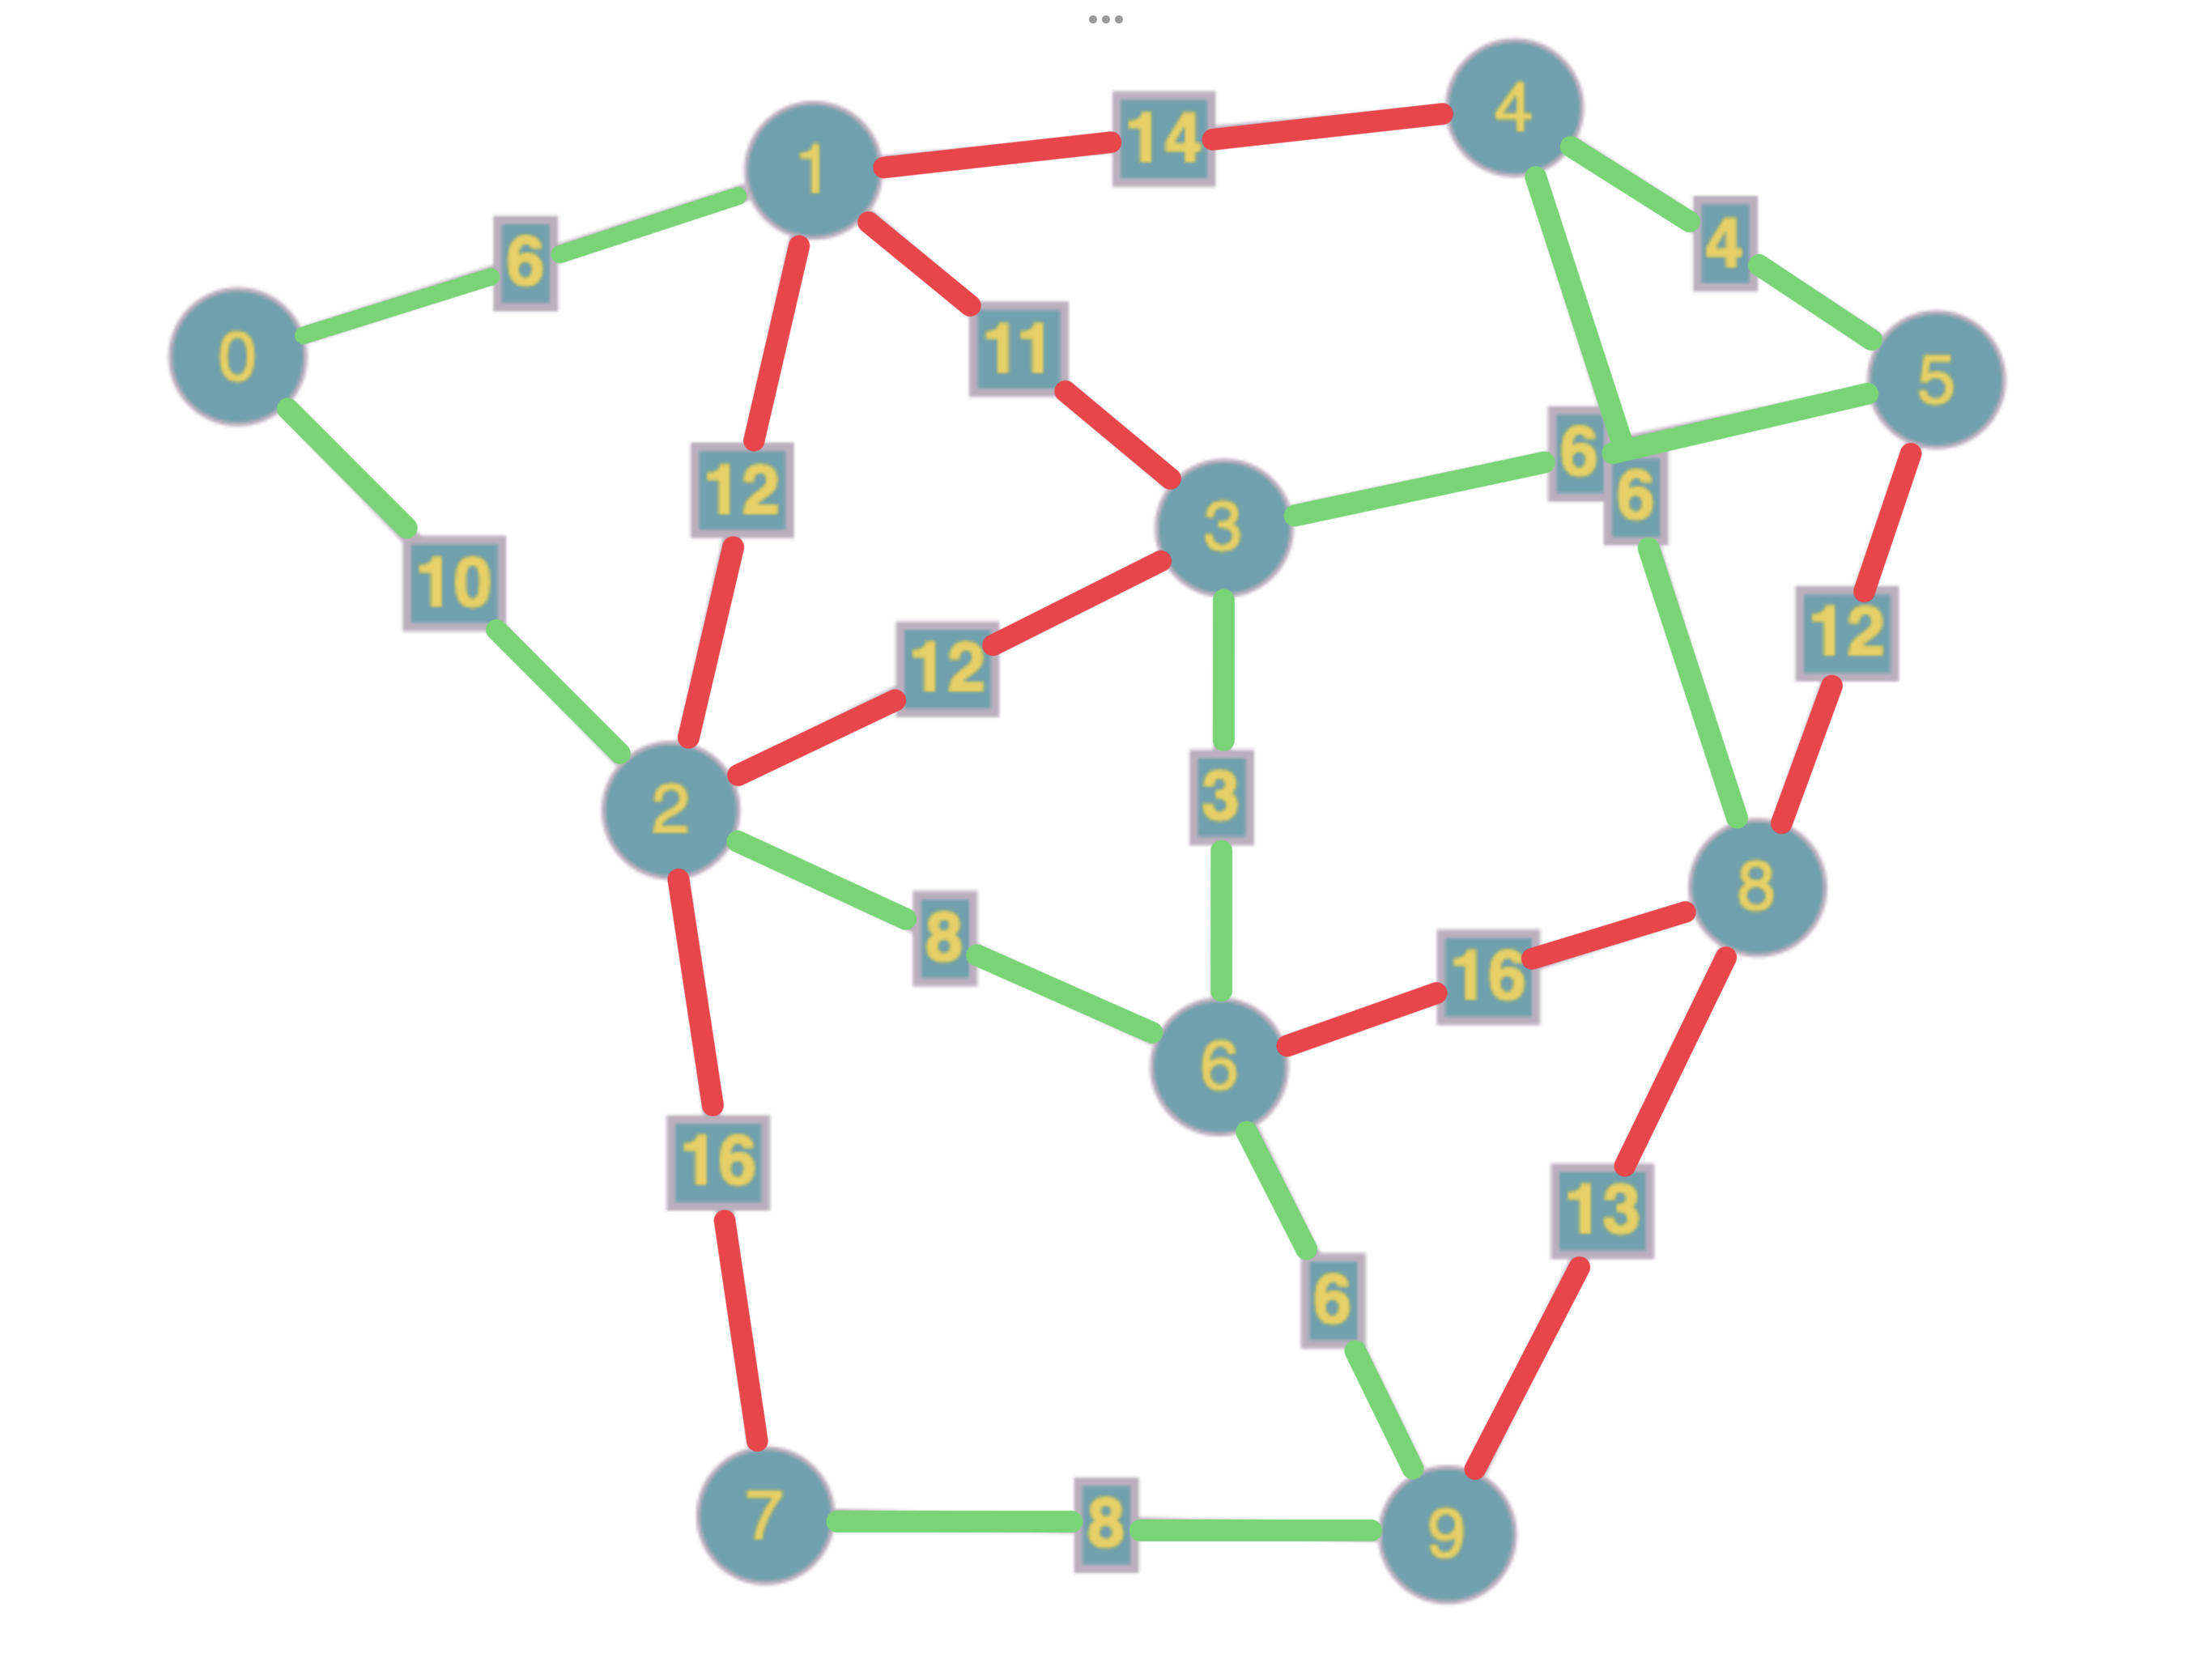
\includegraphics[width=\textwidth]{colorizedMST.jpeg}
\end{center}

\section{Question 3}

Please go to the next page to see the Pseudocode for Question 3.
When a node is deleted from a heap, the other nodes must be rearranged in order to continue to meet the requirements of a heap (the data value at the root of a heap is larger than all of its children). Therefore, an algorithm that finds and deletes the element of the smallest value in a heap also needs to rearrange the surrounding nodes in order for the remaining data structure to continue to be classified as a heap. The siftdown algorithm accomplishes just this. The siftdown algorithm moves a new data item in a child branch down to the correct location in the heap in order to re-establish the heap. The algorithm must first identify the smallest element in the heap, remove that element from the heap, and then use the siftdown algorithm to re-establish the conditions of the heap. The time efficiency of the following algorithm is O(n).   
\begin{algorithm}
\caption{deleteNode}\label{alg:cap}
\begin{algorithmic}
\If{$(heap \ is \ empty)$}
\State \Return false
\Else
\State $size \gets sizeof(arr) / sizeof(arr[0])$
\State $N \gets size(heap)$
\State $minElement \gets heap[\frac{N}{2}]$
\For{$i \gets \frac{n}{2+1} until \ n$}
\State $minElement \gets min(minElement, heap[i])$
\EndFor
\For{$i \gets 1 \ until \ n$}
\If{$(heap[i]=minElement)$}
\State $M \gets i$
\State $heap[i] \gets heap[M]$
\EndIf
\EndFor
\For{$i \gets m \ unitl \ \frac{2}{n}$}
\If{$(heap[2 \times i] > heap[(2 \times i) + 1] \ and \  heap[2 \times i] > heap[i])$}
\State $swap(heap[i], heap[2 \times i])$
\State $i \gets (2 \times i)+1$
\ElsIf{$(heap[2 \times i] < heap[(2 \times i)+1] \ and \  heap[(2 \times i)+1] > heap[i]$)}
\State $swap(heap[i], heap[(2 \times i)+1]$)
\State $i \gets (2 \times i)+1$
\Else
\State break
\EndIf
\EndFor
\State $n \gets n-1$
\EndIf
\end{algorithmic}
\end{algorithm}

\begin{algorithm}
\caption{correctHeap}\label{alg:cap}
\begin{algorithmic}
\State $index \gets 1$
\While{$(index < size)$}
\State $siftdown(heap, index)$
\State $index++$
\EndWhile
\end{algorithmic}
\end{algorithm}

\begin{algorithm}
\caption{siftdown}\label{alg:cap}
\begin{algorithmic}
\State $leftchildindex \gets root \times 2+1$
\State $rightchildindex \gets root \times 2+2$
\If{$(leftchildindex <= last)$}
\State $leftkey \gets heap[leftchildindex].key$
\If{$(rightchildindex <= last)$}
\State $rightkey \gets heap[rightchildindex].key$
\Else
\State $rightkey \gets leftkey-1$
\EndIf
\If{$(leftkey > rightkey)$}
\State $largerchildkey \gets leftkey$
\State $largerchildindex \gets leftchildindex$
\Else
\State $largerchildkey \gets rightkey$
\State $largerchildindex \gets rightchildindex$
\EndIf
\If{$(heap[root].key < largerchildkey)$}
\State $swap(heap, root, largerchildindex)$
\State $siftdown(heap, largerchildindex, last)$
\EndIf
\EndIf
\end{algorithmic}
\end{algorithm}

\paragraph{\linebreak I declare that all material in this assessment task is my work except where there is clear acknowledgment or reference to the work of others. I further declare that I have complied and agreed to the CMU Academic Integrity Policy at the University website.
\linebreak  http://www.coloradomesa.edu/student-services/documents
\linebreak \linebreak Author’s Name: Mia Weber UID: 700510845 Date: 10/30/2022
\linebreak Author's Name: Brandon Kamplain UID: 700510289 Date: 10/30/2022}


\end{document}